\chapter{Dot Product}

Let $\vec{v} = \langle v_1, v_2, v_3 \rangle$ and $\vec{u} = \langle u_1, u_2,
    u_3 \rangle$ be two vectors in $\mathbb{R}^3$ (three-dimensional space), then
the dot product of $\vec{v}$ and $\vec{u}$ is given by \[\vec{v} \cdot \vec{u} = v_1u_1 + v_2u_2 + v_3u_3\]
The final result of the dot product is a number, hence the name \textbf{scalar
    product}. The dot product is also known as the \textbf{inner product} of two
vectors.

~\\ \noindent\textbf{Example 1. } Calculate the dot product of the
vectors $\vec{v} = \langle 1, 2 \rangle$ and $\vec{u} = \langle -2, 1 \rangle$.
\begin{align*}
    \vec{v} \cdot \vec{u} & = v_1u_1 + v_2u_2 \\
                          & = 1(-2) + 2(1)    \\
                          & = 0
\end{align*}
\begin{framed}
    \noindent\textbf{Note: }

    \noindent If $\vec{v} \cdot \vec{u} = 0$, then $\vec{v}$ and $\vec{u}$ are perpendicular to each other, or they are \textbf{orthogonal}. That is,
    \[\vec{v} \cdot \vec{u} = 0 \Longleftrightarrow \vec{v} \perp \vec{u}\]
\end{framed}
\newpage
\section*{Properties of Dot Product}
\begin{enumerate}[leftmargin=*]
    \item $\vec{v} \cdot \vec{u} = \vec{u} \cdot \vec{v}$
    \item $\vec{v} \cdot (\vec{u} + \vec{w}) = \vec{v} \cdot \vec{u} + \vec{v} \cdot \vec{w}$
    \item $(c\vec{v}) \cdot \vec{u} = c(\vec{v} \cdot \vec{u})$, where $c$ is a scalar
    \item $\vec{0}\cdot\vec{v} = 0$, where $\vec{0} = \langle 0, 0 \rangle$
    \item $\vec{v} \cdot \vec{v} = \norm{\vec{v}}^2$
    \item The angle $\theta$ between two vectors $\vec{v}$ and $\vec{u}$ is given by \[\cos\theta = \frac{\vec{u} \cdot \vec{v}}{\norm{\vec{u}} \norm{\vec{v}}} \qquad \text{where} \qquad 0 \leq \theta \leq \pi\]
          From this, we can easily derive that
    \item $\vec{u} \cdot \vec{v} = \norm{\vec{u}} \norm{\vec{v}} \cos\theta$
\end{enumerate}
\noindent\textbf{Example 1. } Let $\vec{v} = \langle 1, 2 \rangle$, $\vec{u} = \langle 3, 4 \rangle$. Calculate $\vec{u} \cdot (5\vec{v})$.
\begin{align*}
    \vec{u} \cdot (5\vec{v}) & = 5(\vec{u} \cdot \vec{v}) \\
                             & = 5(1 \cdot 3 + 2 \cdot 4) \\
                             & = 55
\end{align*}
\noindent\textbf{Example 2. } Prove property 5.
\\\\
\noindent Let $\vec{v} = \langle v_1, v_2 \rangle$, then
\begin{align*}
    \vec{v} \cdot \vec{v} & = \langle v_1, v_2 \rangle \cdot \langle v_1, v_2 \rangle \\
                          & = v_1v_1 + v_2v_2                                         \\
                          & = v_1^2 + v_2^2                                           \\
                          & = \left(\sqrt{v_1^2 + v_2^2}\right)^2                     \\
                          & = \norm{\vec{v}}^2 \qquad \blacksquare
\end{align*}
\noindent\textbf{Example 3. } Calculate the dot product of the vectors $\vec{v} = \langle 1, 2, 4 \rangle$ and $\vec{u} = \langle -3, -2, 0 \rangle$.
\begin{align*}
    \vec{v} \cdot \vec{v} & = \langle 1, 2, 4 \rangle \cdot \langle -3, -2, 0 \rangle \\
                          & = 1(-3) + 2(-2) + 4(0)                                    \\
                          & = -7
\end{align*}
\noindent\textbf{Example 4. } Calculate the dot product of the vectors $\vec{v} = 3i + 2j + 4k$ and $\vec{u} = -i + j$.
\begin{align*}
    \vec{v} \cdot \vec{u} & = (3i + 2j + 4k) \cdot (-i + j) \\
                          & = 3(-1) + 2(1) + 4(0)           \\
                          & = -1
\end{align*}
\noindent\textbf{Example 5. } Determine whether the following vectors are orthogonal. \[\vec{v} = -2i + 3j + k \qquad \vec{u} = 2i + j + k\]
\begin{align*}
    \vec{v} \cdot \vec{u} & = (-2i + 3j + k) \cdot (2i + j + k) \\
                          & = -2(2) + 3(1) + 1(1)               \\
                          & = 0
\end{align*}
Since $\vec{v} \cdot \vec{u} = 0$, $\vec{v}$ and $\vec{u}$ are orthogonal.

~\\\noindent\textbf{Example 6. } Find the angle between the vectors $\vec{v} = \langle 3, 1 \rangle$ and $\vec{u} = \langle 2, -1 \rangle$.
\begin{align*}
    \cos\theta & = \frac{\vec{u} \cdot \vec{v}}{\norm{\vec{u}} \norm{\vec{v}}} \\
               & = \frac{3(2) + 1(-1)}{\sqrt{3^2 + 1^2}\sqrt{2^2 + (-1)^2}}    \\
               & = \frac{5}{\sqrt{10}\sqrt{5}}                                 \\
               & = \frac{1}{\sqrt{2}}                                          \\
    \theta     & = \cos^{-1}\left(\frac{1}{\sqrt{2}}\right)                    \\
               & = \frac{\pi}{4}
\end{align*}
\noindent\textbf{Example 7. } Find the angle between the vectors $\vec{v} = i - 3j + k$ and $\vec{u} = 2i + 4j - k$.
\begin{align*}
    \cos\theta & = \frac{\vec{u} \cdot \vec{v}}{\norm{\vec{u}} \norm{\vec{v}}}                       \\
               & = \frac{1(2) + (-3)(4) + 1(-1)}{\sqrt{1^2 + (-3)^2 + 1^2}\sqrt{2^2 + 4^2 + (-1)^2}} \\
               & = \frac{-11}{\sqrt{231}}                                                            \\
    \theta     & = 2.38 \text{ rad}
\end{align*}

\newpage

\section*{Selected Exercises}
\textit{Source: Thomas' Calculus 14th Ed. Exercise 11.3}

\subsection*{Theory and Examples}

\begin{enumerate}
    \setcounter{enumi}{18}
    \item \textbf{Sums and differences} In the accompanying figure, it looks as if
          $\mathbf{v}_1+\mathbf{v}_2$ and $\mathbf{v}_1-\mathbf{v}_2$ are orthogonal. Is
          this mere coincidence, or are there circumstances under which we may expect the
          sum of two vectors to be orthogonal to their difference? Give reasons for your
          answer. \begin{center}
              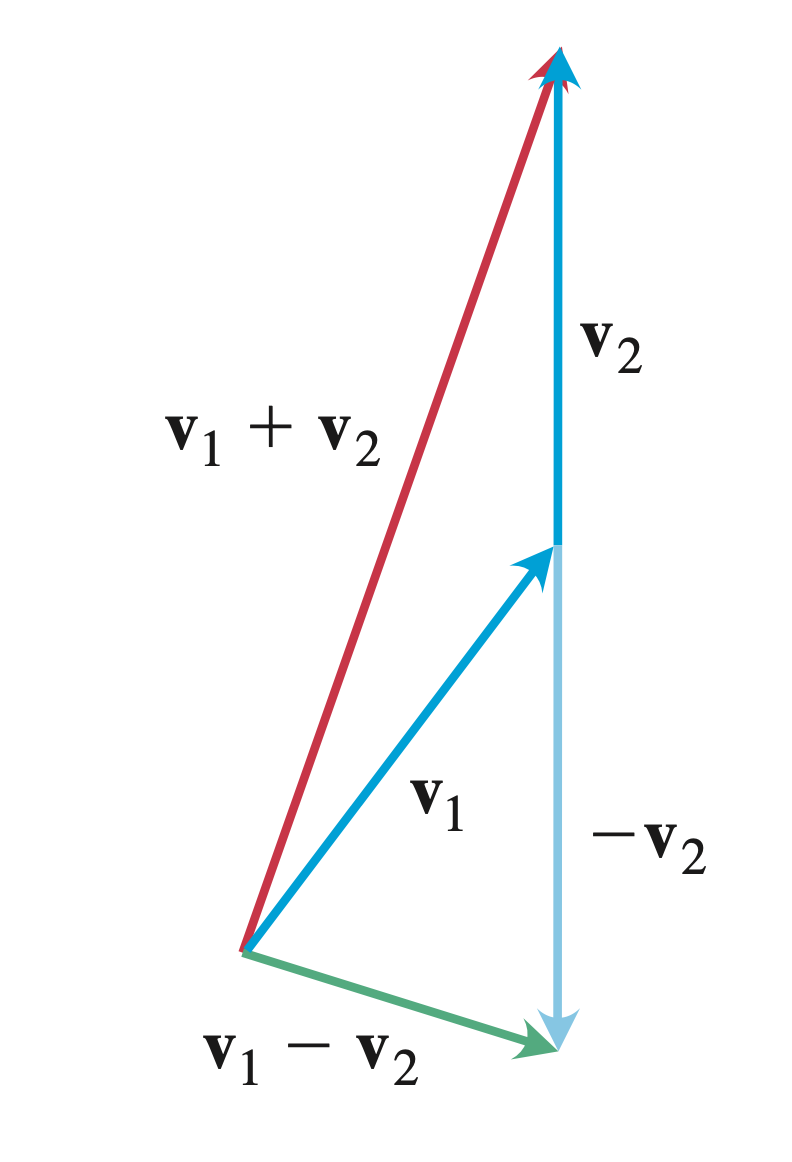
\includegraphics[scale=0.3]{./assets/thomas12.3q19.png}
          \end{center}

          \sol{}
          \begin{align*}
              (v_1 + v_2) \cdot (v_1 - v_2) & = v_1 \cdot v_1 - v_1 \cdot v_2 + v_2 \cdot v_1 - v_2 \cdot v_2 \\
                                            & = \norm{v_1}^2 - \norm{v_2}^2                                   \\
                                            & = 0 \quad (v_1 = v_2)
          \end{align*}
          Therefore, the sum of two vectors is orthogonal to their difference \textbf{if and only if the two vectors are in equal length}. $\hfill\blacksquare$

          \newpage
    \item \textbf{Orthogonality on a circle} Suppose that $A B$ is the diameter of a circle with
          center $O$ and that $C$ is a point on one of the arcs joining $A$ and $B$. Show
          that $\overrightarrow{C A}$ and $\overrightarrow{C B}$ are orthogonal.
          \begin{center}
              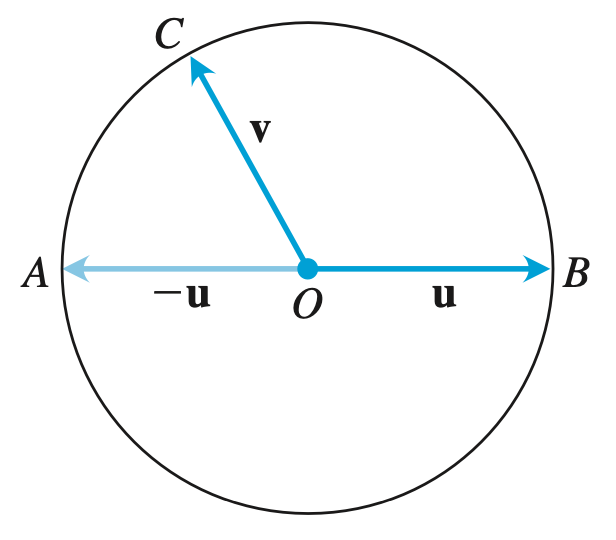
\includegraphics[scale=0.4]{./assets/thomas12.3q20.png}
          \end{center}
          \sol{} Since $\norm{u} = \norm{v} = $ radius of the circle, $\overrightarrow{C A} = \overrightarrow{CO} + \overrightarrow{OA} = -u - v$ and $\overrightarrow{C B} = \overrightarrow{CO} + \overrightarrow{OB} = u - v$, we have
          \begin{align*}
              \overrightarrow{C A} \cdot \overrightarrow{C B} & = (-u - v) \cdot (u - v)                               \\
                                                              & = -u \cdot u - u \cdot (-v) - v \cdot u - v \cdot (-v) \\
                                                              & = -\norm{u}^2 + \norm{v}^2                             \\
                                                              & = 0
          \end{align*}
          Therefore, $\overrightarrow{C A}$ and $\overrightarrow{C B}$ are orthogonal. $\hfill\blacksquare$

    \item \textbf{Diagonals of a rhombus} Show that the diagonals of a rhombus (parallelogram with
          sides of equal length) are perpendicular.
          \sol{}
          \begin{center}
              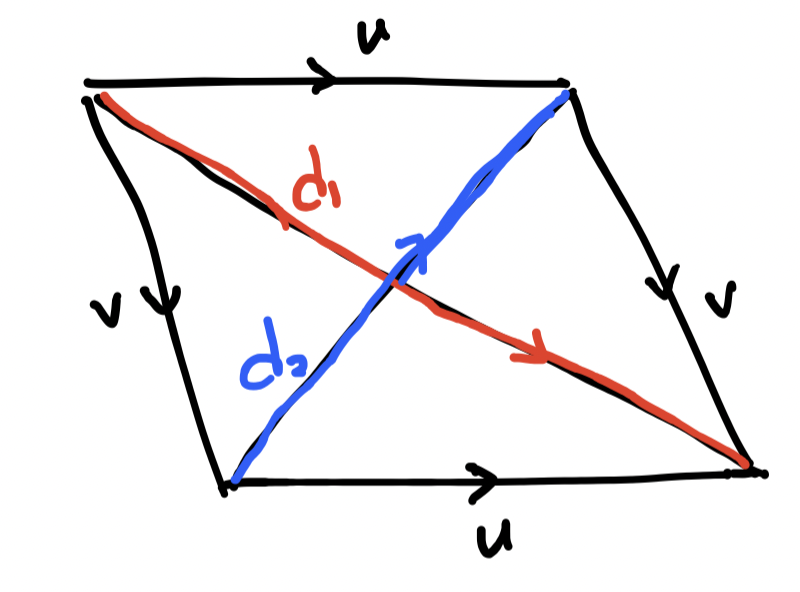
\includegraphics[scale=0.4]{assets/thomas12.3q21.png}
          \end{center}
          Since $d_1 = u + v$ and $d_2 = -v + u$, we have
          \begin{align*}
              d_1 \cdot d_2 & = (u + v) \cdot (-v + u)                        \\
                            & = u \cdot u - u \cdot v + v \cdot u - v \cdot v \\
                            & = \norm{u}^2 - \norm{v}^2                       \\
                            & = 0
          \end{align*}
          Therefore, the diagonals of a rhombus are perpendicular. $\hfill\blacksquare$

          \setcounter{enumi}{23}
    \item \textbf{Diagonal of parallelogram} Show that the indicated diagonal of the parallelogram
          determined by vectors $\mathbf{u}$ and $\mathbf{v}$ bisects the angle between
          $\mathbf{u}$ and $\mathbf{v}$ if $|\mathbf{u}|=|\mathbf{v}|$.
          \begin{center}
              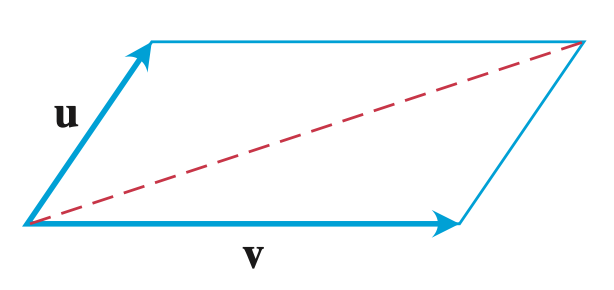
\includegraphics[scale=0.5]{assets/thomas12.3q24.png}
          \end{center}
          \text{Solution. }
          \begin{align*}
              (u + v) \cdot u & = u \cdot u + u \cdot v  \\
                              & = \norm{u}^2 + u \cdot v \\
                              & = \norm{v}^2 + u \cdot v \\
                              & = v \cdot v + u \cdot v  \\
                              & = (u + v) \cdot v
          \end{align*}
          Hence, the angle $\arccos\left(\dfrac{(u + v) \cdot u}{\norm{u + v} \norm{u}}\right)$ between the diagonal and $\vec{u}$ is equal to the angle $\arccos\left(\dfrac{(u + v) \cdot v}{\norm{u + v} \norm{v}}\right)$ between the diagonal and $\vec{v}$ because the inverse cosine function is one-to-one.

          Therefore, the indicated diagonal of the parallelogram determined by vectors
          $\mathbf{u}$ and $\mathbf{v}$ bisects the angle between $\mathbf{u}$ and
          $\mathbf{v}$ if $|\mathbf{u}|=|\mathbf{v}|$. $\hfill\blacksquare$

    \item \textbf{Projectile motion} A gun with muzzle velocity of $400 \mathrm{~m} / \mathrm{s}$ is fired at an angle of $8^{\circ}$ above the horizontal. Find the horizontal and vertical components of the velocity.
          \sol{} Let $\vec{v + u}$ be the velocity of the bullet, where $\vec{v}$ is the vertical component and $\vec{u}$ is the horizontal component.
          \begin{multicols}{2}
              \begin{center}
                  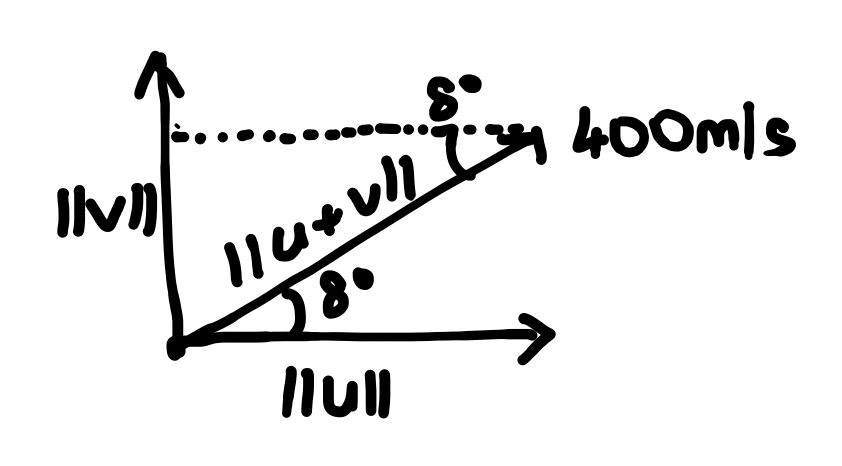
\includegraphics[scale=0.5]{assets/thomas12.3q25.png}
              \end{center}
              \columnbreak
              \begin{align*}
                  \dfrac{\norm{u}}{\norm{u + v}} & = \cos 8^{\circ}                   \\
                  \norm{u}                       & = 400 \cos 8^{\circ}               \\
                                                 & = 396.107 \mathrm{~m} / \mathrm{s}
              \end{align*}

              \begin{align*}
                  \dfrac{\norm{v}}{\norm{u + v}} & = \sin 8^{\circ}                  \\
                  \norm{v}                       & = 400 \sin 8^{\circ}              \\
                                                 & = 55.669 \mathrm{~m} / \mathrm{s}
              \end{align*}
              $\hfill\blacksquare$

          \end{multicols}

    \item \textbf{Inclined plane} Suppose that a box is being towed up an inclined plane as shown in the figure. Find the force $w$ needed to make the component of the force parallel to the inclined plane equal to $2.5 \mathrm{~N}$.
          \begin{center}
              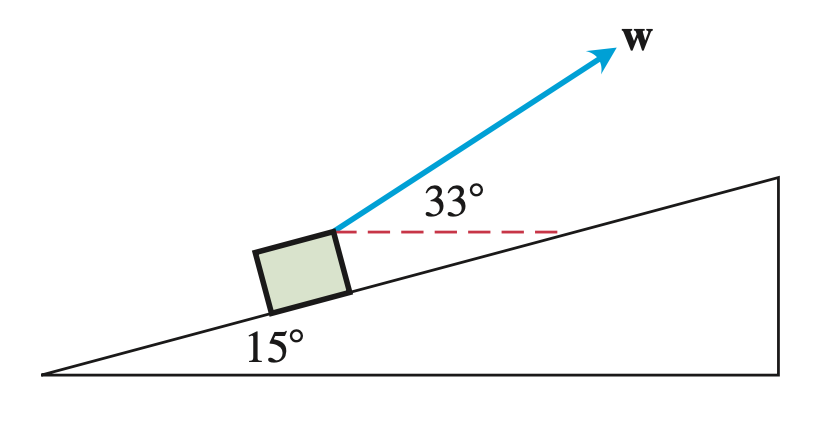
\includegraphics[scale=0.5]{assets/thomas12.3q26.png}
          \end{center}
          \sol{}
          \begin{center}
              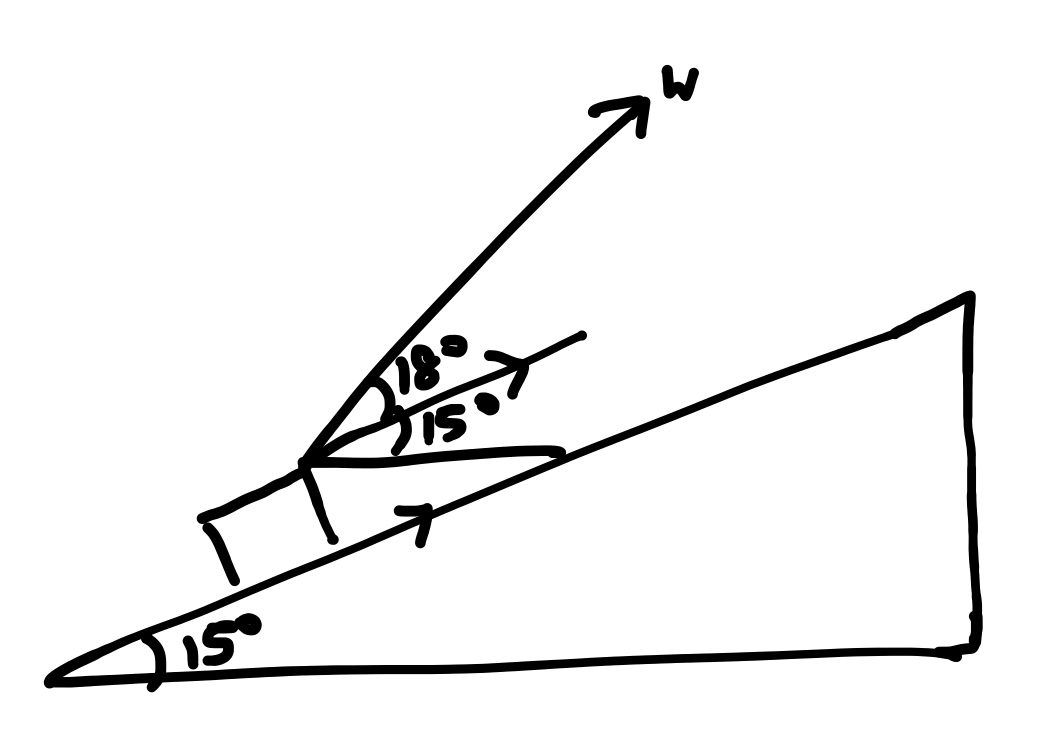
\includegraphics[scale=0.4]{assets/thomas12.3q26sol.png}
          \end{center}
          \begin{align*}
              \norm{w} \cos (33^{\circ} - 15^{\circ}) & = 2.5                          \\
              \norm{w}                                & = \dfrac{2.5}{\cos 18^{\circ}}
          \end{align*}
          \begin{align*}
              w & = \norm{w} \langle \cos 33^{\circ}, \sin 33^{\circ} \rangle                    \\
                & =\dfrac{2.5}{\cos 18^{\circ}} \langle \cos 33^{\circ}, \sin 33^{\circ} \rangle \\
                & = \langle 2.205, 1.432 \rangle                                                 \\
          \end{align*}

          $\hfill\blacksquare$

          \textit{\textbf{Note: } This question can be solved solely by using trigonometry.}

          \newpage
          \setcounter{enumi}{28}
    \item \textbf{Orthogonal unit vectors} If $\mathbf{u}_1$ and $\mathbf{u}_2$ are orthogonal unit vectors and $\mathbf{v}=a \mathbf{u}_1+b \mathbf{u}_2$, find $\mathbf{v} \cdot \mathbf{u}_1$.
          \sol{}
          \begin{align*}
              \mathbf{v} \cdot \mathbf{u}_1 & = (a \mathbf{u}_1+b \mathbf{u}_2) \cdot \mathbf{u}_1                  \\
                                            & = a \mathbf{u}_1 \cdot \mathbf{u}_1+b \mathbf{u}_2 \cdot \mathbf{u}_1 \\
                                            & = a \norm{\mathbf{u}_1}^2 + b \mathbf{u}_2 \cdot \mathbf{u}_1         \\
                                            & = a(1) + b(0)                                                         \\
                                            & = a
          \end{align*}
          $\hfill\blacksquare$

    \item A force $\mathbf{F}=2 \mathbf{i}+\mathbf{j}-3 \mathbf{k}$ is applied to a
          spacecraft with velocity vector $\mathbf{v}=3 \mathbf{i}-\mathbf{j}$. Express
          $\mathbf{F}$ as a sum of a vector parallel to $\mathbf{v}$ and a vector
          orthogonal to $\mathbf{v}$. \sol{} The vector parallel to $\mathbf{v}$ is
          \begin{align*}
              \text{proj}_v F & = \left(\dfrac{F \cdot v}{\norm{v}^2}\right)v             \\
                              & = \left(\dfrac{5}{10}\right)(3i - j)                      \\
                              & = \left(\dfrac{3}{2}\right)i - \left(\dfrac{1}{2}\right)j
          \end{align*}
          The vector orthogonal to $\mathbf{v}$ is
          \begin{align*}
              \mathbf{F} - \text{proj}_v F & = \left(2i + j - 3k\right) - \left(\dfrac{3}{2}\right)i + \left(\dfrac{1}{2}\right)j \\
                                           & = \left(\dfrac{1}{2}\right)i + \left(\dfrac{3}{2}\right)j - 3k
          \end{align*}
          $\hfill\blacksquare$

\end{enumerate}

\subsection*{Equations for Lines in the Plane}

\begin{enumerate}
    \setcounter{enumi}{32}
    \item \textbf{Line perpendicular to a vector} Show that $\mathbf{v}=a \mathbf{i}+b \mathbf{j}$ is perpendicular to the line $a x+b y=c$ by establishing that the slope of the vector $\mathbf{v}$ is the negative reciprocal of the slope of the given line.
          \sol{} Let $P(x_1, y_1)$ and $Q(x_2, y_2)$ be two points on the line $ax + by = c$. Then,
          \begin{align*}
              P(x_1, y_1) & = \left(x_1, \dfrac{c - ax_1}{b}\right) \\
              Q(x_2, y_2) & = \left(x_2, \dfrac{c - ax_2}{b}\right)
          \end{align*}
          \begin{align*}
              \overrightarrow{PQ} & = \left\langle x_2 - x_1, y_2 - y_1 \right\rangle                                 \\
                                  & = \left\langle x_2 - x_1, \dfrac{c - ax_2}{b} - \dfrac{c - ax_1}{b} \right\rangle \\
                                  & = \left\langle x_2 - x_1, \dfrac{a(x_1 - x_2)}{b} \right\rangle
          \end{align*}
          \begin{align*}
              \overrightarrow{PQ} \cdot v & = \left\langle x_2 - x_1, \dfrac{a(x_1 - x_2)}{b} \right\rangle \cdot \left\langle a, b \right\rangle \\
                                          & = a(x_2 - x_1) + \dfrac{a(x_1 - x_2)}{b} \cdot b                                                      \\
                                          & = a(x_2 - x_1) - a(x_2 - x_1)                                                                         \\
                                          & = 0
          \end{align*}
          Therefore, $\mathbf{v}$ is perpendicular to the line $ax + by = c$. $\hfill\blacksquare$
          ~\\\\
          Alternatively, the slope of the vector $\mathbf{v}$ is $\dfrac{b}{a}$, while
          the slope of the line $ax + by = c$ is $-\dfrac{a}{b}$. Therefore, the vector
          $\mathbf{v}$ is perpendicular to the line $ax + by = c$, since slope of the vector $\mathbf{v}$ is the negative reciprocal of the slope of the given line. $\hfill\blacksquare$

    \item \textbf{Line parallel to a vector} Show that the vector $\mathbf{v}=a \mathbf{i}+b \mathbf{j}$ is parallel to the line $b x-a y=c$ by establishing that the slope of the line segment representing $\mathbf{v}$ is the same as the slope of the given line.
          \sol{} The slope of the vector $v$ is $\dfrac{b}{a}$, while the slope of the given line is also $\dfrac{b}{a}$. Therefore, the vector $\mathbf{v}$ is parallel to the line $bx - ay = c$. $\hfill\blacksquare$
\end{enumerate}

\subsection*{Work}

\begin{enumerate}
    \setcounter{enumi}{42}
    \item \textbf{Work along a line} Find the work done by a force $\mathbf{F}=5 \mathbf{i}$
          (magnitude $5 \mathrm{~N}$) in moving an object along the line from the origin
          to the point $(1,1)$ (distance in meters).
          \sol{} Let $\vec{D} = \langle 1, 1 \rangle$ be the displacement vector of the object.
          \begin{align*}
              W & = \vec{F} \cdot \vec{D} \\
                & = <5, 0> \cdot <1, 1>   \\
                & = 5 \mathrm{~J}
          \end{align*}
    \item \textbf{Locomotive The Union Pacific's Big Boy} locomotive could pull 6000-tonne trains
          with a tractive effort (pull) of 602,148 N. At this level of effort, about how
          much work did Big Boy do on the (approximately straight) $605-\mathrm{km}$
          journey from San Francisco to Los Angeles?
          \sol{}
          \begin{align*}
              W & = \vec{F} \cdot \vec{D}                     \\
                & = \norm{\vec{F}} \norm{\vec{D}} \cos \theta \\
                & = 602148 \cdot 605000 \cdot \cos 0^{\circ}  \\
                & = 3.6429954 \times 10^{11} \mathrm{~J}
          \end{align*}
          $\hfill\blacksquare$

    \item \textbf{Inclined plane} How much work does it take to slide a crate $20 \mathrm{~m}$
          along a loading dock by pulling on it with a $200$N force at an angle
          of $30^{\circ}$ from the horizontal?
          \sol{}
          \begin{align*}
              W & = \vec{F} \cdot \vec{D}                     \\
                & = \norm{\vec{F}} \norm{\vec{D}} \cos \theta \\
                & = 200 \cdot 20 \cdot \cos 30^{\circ}        \\
                & = 3464.102 \mathrm{~J}
          \end{align*}
          $\hfill\blacksquare$

    \item \textbf{Sailboat} The wind passing over a boat's sail exerted a $1000 \mathrm{~N}$
          magnitude force $\mathbf{F}$ as shown here. How much work did the wind perform
          in moving the boat forward $1 \mathrm{~km}$? Answer in joules.
          \begin{center}
              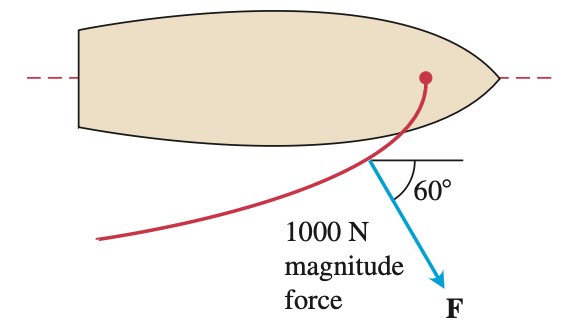
\includegraphics[scale=0.6]{assets/thomas12.3q46.png}
          \end{center}
          \sol{}
          \begin{align*}
              W & = \vec{F} \cdot \vec{D}                     \\
                & = \norm{\vec{F}} \norm{\vec{D}} \cos \theta \\
                & = 1000 \cdot 1000 \cdot \cos 60^{\circ}     \\
                & = 500000 \mathrm{~J}
          \end{align*}
          $\hfill\blacksquare$
\end{enumerate}

\newpage
\section*{Selected Exercises}
\textit{Source: Larson Calculus 11th Ed. Exercise 11.3}

\begin{enumerate}
    \setcounter{enumi}{54}
    \item \textbf{Finding an Angle} Find the angle between a cube's diagonal and one of its edges.
          \sol{} Let $a$ be the length of the cube's edge, then the length of the cube's diagonal is $\sqrt{3}a$. Let one side of the cube $\vec{u} = \langle a, 0, 0 \rangle$ and the diagonal of the cube $\vec{v} = \langle a, a, a \rangle$, then
          \begin{align*}
              \cos\theta & = \frac{\vec{u} \cdot \vec{v}}{\norm{\vec{u}} \norm{\vec{v}}} \\
                         & = \frac{a^2 + 0 + 0}{a\sqrt{3}a}                              \\
                         & = \frac{1}{\sqrt{3}}                                          \\
              \theta     & = \arccos\left(\frac{1}{\sqrt{3}}\right)                      \\
                         & = 54.74^{\circ}
          \end{align*}
          $\hfill\blacksquare$

    \item \textbf{Finding an Angle} Find the angle between the diagonal of a cube and the diagonal of one of its sides.
          \sol{} Let $a$ be the length of the cube's edge, then the length of the cube's diagonal is $\sqrt{3}a$, and the length of the diagonal of one of its sides is $\sqrt{2}a$. Let the diagonal of the cube $\vec{u} = \langle a, a, a \rangle$ and the diagonal of one of its sides $\vec{v} = \langle a, a, 0 \rangle$, then
          \begin{align*}
              \cos\theta & = \frac{\vec{u} \cdot \vec{v}}{\norm{\vec{u}} \norm{\vec{v}}} \\
                         & = \frac{a^2 + a^2 + 0}{\sqrt{3}a\sqrt{2}a}                    \\
                         & = \frac{2}{\sqrt{6}}                                          \\
              \theta     & = \arccos\left(\frac{2}{\sqrt{6}}\right)                      \\
                         & = 35.26^{\circ}
          \end{align*}
          $\hfill\blacksquare$

          \newpage
    \item \textbf{Braking Load} A truck weighing 22 metric tons is parked on a $10^{\circ}$ slope (see figure). Assume the only force to overcome is that due to gravity. Find (a) the force required to keep the truck from rolling down the hill and (b) the force perpendicular to the hill.
          \sol{}
          \begin{enumerate}[label=(\alph*)]
              \item \begin{center}
                        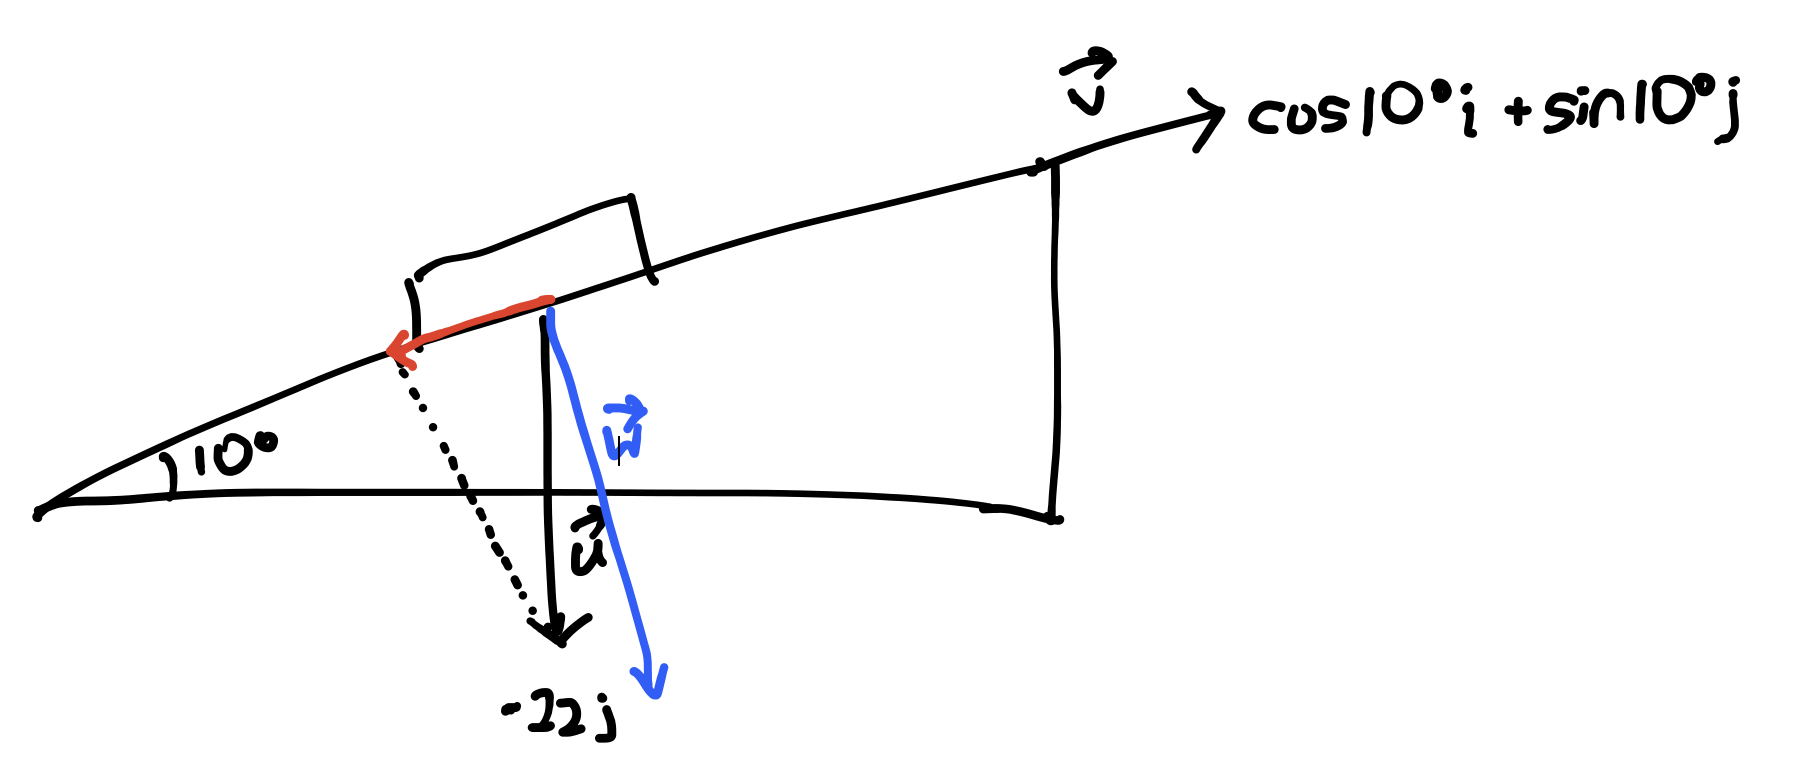
\includegraphics[scale=0.4,valign=t]{assets/larson11.3q57.png}
                    \end{center}
                    Let $\vec{F}$ be the force required for the truck to roll down the hill, then $\vec{F}$ is the projection of the force due to gravity $\vec{u} = \langle 0, -22000 \rangle$ onto the hill $\vec{v} = \langle \cos 10^{\circ}, \sin 10^{\circ} \rangle$.
                    \begin{align*}
                        \vec{F} & = \text{proj}_{\vec{v}}\vec{u}                                                              \\
                                & = \left(\frac{\vec{u} \cdot \vec{v}}{\norm{\vec{v}}^2}\right)\vec{v}                        \\
                                & = \frac{(-22000)(\sin 10^{\circ})}{1}\cdot \langle \cos 10^{\circ}, \sin 10^{\circ} \rangle \\
                                & = -3820.26\langle \cos 10^{\circ}, \sin 10^{\circ} \rangle
                    \end{align*}
                    Since a force of $\norm{F} = 3.82$ metric tons is required for the truck to roll down the hill, the same force of $3.82$ metric tons is required to keep the truck from rolling down the hill. $\hfill\blacksquare$

              \item Let $\vec{w}$ be the force perpendicular to the hill, then
                    \begin{align*}
                        \vec{u}  & = \vec{F} + \vec{w}                                                                                       \\
                        \vec{w}  & = \vec{u} - \vec{F}                                                                                       \\
                                 & = \langle 0, -22000 \rangle - ((-22000)(\sin 10^{\circ})\langle \cos 10^{\circ}, \sin 10^{\circ} \rangle) \\
                                 & = \langle 22000(\sin 10^{\circ})\cos 10^{\circ}, -22000 + 22000\sin 10^{\circ}\sin 10^{\circ} \rangle     \\
                                 & = \langle 3762.222, -21336.619 \rangle                                                                    \\
                        \norm{w} & = \sqrt{(3762.222)^2 + (-21336.619)^2}                                                                    \\
                                 & = 21.67 \text{ metric tons}
                    \end{align*}
                    $\hfill\blacksquare$
          \end{enumerate}

          \setcounter{enumi}{58}

          \newpage
    \item Work An object is pulled 10 meters across a floor using a force of 85 newtons.
          The direction of the force is $60^{\circ}$ above the horizontal (see figure).
          Find the work done.
          \begin{center}
              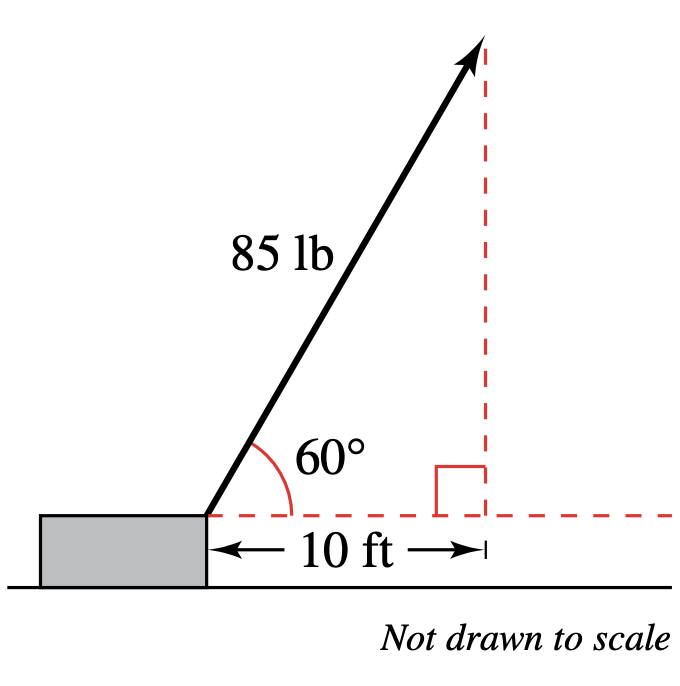
\includegraphics[scale=0.4,valign=t]{assets/larson11.3q59.png}
          \end{center}
          \sol{} Let $\vec{F} = \langle 85 \cos 60^{\circ}, 85 \sin 60^{\circ} \rangle$ be the force applied to the object, and $\vec{D} = \langle 10, 0 \rangle$ be the displacement vector of the object, then
          \begin{align*}
              W & = \vec{F} \cdot \vec{D}                                                              \\
                & = \langle 85 \cos 60^{\circ}, 85 \sin 60^{\circ} \rangle \cdot \langle 10, 0 \rangle \\
                & = 425 \text{ joules}
          \end{align*}
          \setcounter{enumi}{60}
    \item Work A car is towed using a force of 1600 newtons. The chain used to pull the
          car makes a $25^{\circ}$ angle with the horizontal. Find the work done in
          towing the car 2 kilometers.
          \begin{center}
              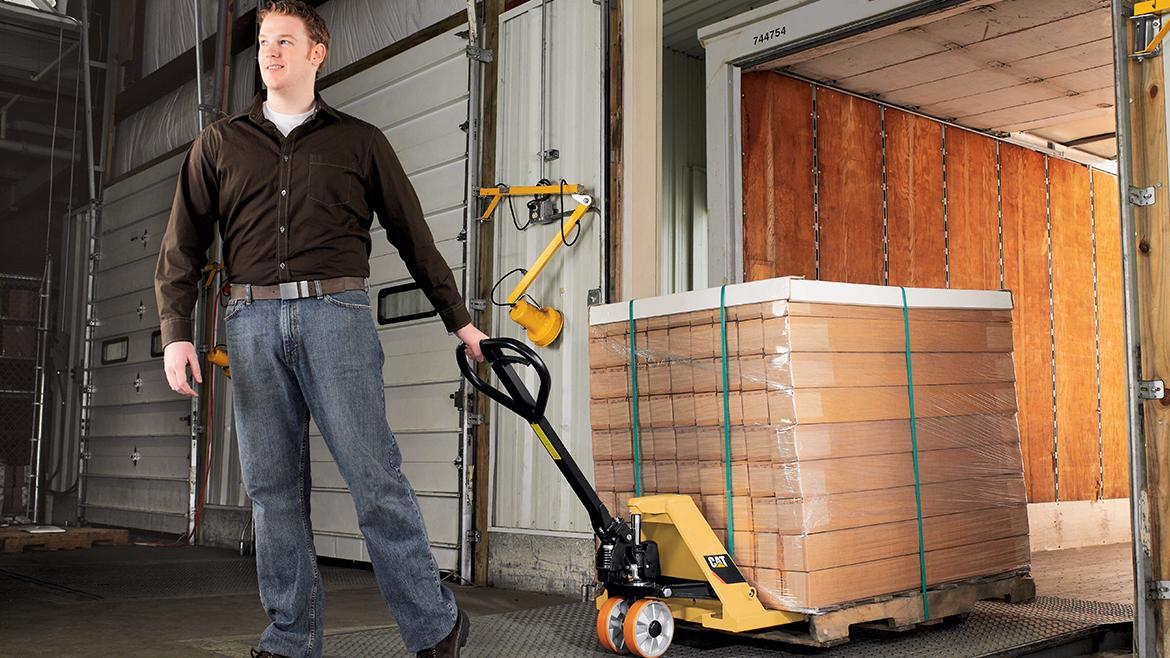
\includegraphics[scale=0.2,valign=t]{assets/larson11.3q61.jpg}
          \end{center}
          \sol{} Let $\vec{F} = \langle 1600 \cos
              25^{\circ}, 1600 \sin 25^{\circ} \rangle$ be the force applied to the car, and
          $\vec{D} = \langle 2000, 0 \rangle$ be the displacement vector of the car, then
          \begin{align*}
              W & = \vec{F} \cdot \vec{D}                                                                    \\
                & = \langle 1600 \cos 25^{\circ}, 1600 \sin 25^{\circ} \rangle \cdot \langle 2000, 0 \rangle \\
                & = 2900 \text{ kJ}
          \end{align*}
          $\hfill\blacksquare$

          \setcounter{enumi}{69}

          \newpage
    \item \textbf{Proof} Use vectors to prove that a parallelogram is a rectangle if and only if its diagonals are equal in length.

          \prooff{}

          \begin{center}
              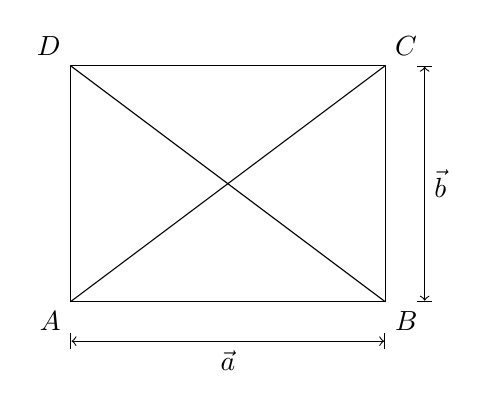
\begin{tikzpicture}
                  \draw (0, 0) -- (4, 0) -- (4, 3) -- (0, 3) -- cycle;
                  \draw (0, 0) -- (4, 3);
                  \draw (0, 3) -- (4, 0);
                  \draw[|<->|] (0, -0.5) -- (4, -0.5) node[midway, below] {$\vec{a}$};
                  \draw[|<->|] (4.5, 0) -- (4.5, 3) node[midway, right] {$\vec{b}$};
                  \node[below left] at (0, 0) {$A$};
                  \node[below right] at (4, 0) {$B$};
                  \node[above right] at (4, 3) {$C$};
                  \node[above left] at (0, 3) {$D$};
              \end{tikzpicture}
          \end{center}

          Let $\vec{a} = \overrightarrow{AB} = \overrightarrow{CD}$ and $\vec{b} = \overrightarrow{AD} = \overrightarrow{BC}$ be the diagonals of the parallelogram $ABCD$ (Opposite sides of a parallelogram are congruent). Let $\overrightarrow{d1} = \overrightarrow{AC}$ and $\overrightarrow{d2} = \overrightarrow{BD}$ be the diagonals of the parallelogram $ABCD$.
          \begin{align*}
              \overrightarrow{d1} = \overrightarrow{AB} + \overrightarrow{BC} & = \vec{a} + \vec{b} \\
              \overrightarrow{d2} = \overrightarrow{BC} + \overrightarrow{CD} & = \vec{b} - \vec{a}
          \end{align*}

          Assume that the diagonals of the parallelogram $ABCD$ are equal in length, then
          \begin{align*}
              \norm{\overrightarrow{d1}}                                             & = \norm{\overrightarrow{d2}}                                             \\
              \overrightarrow{d1} \cdot \overrightarrow{d1}                          & = \overrightarrow{d2} \cdot \overrightarrow{d2}                          \\
              (\vec{a} + \vec{b}) \cdot (\vec{a} + \vec{b})                          & = (\vec{b} - \vec{a}) \cdot (\vec{b} - \vec{a})                          \\
              \vec{a} \cdot \vec{a} + 2\vec{a} \cdot \vec{b} + \vec{b} \cdot \vec{b} & = \vec{b} \cdot \vec{b} - 2\vec{a} \cdot \vec{b} + \vec{a} \cdot \vec{a} \\
              4\vec{a} \cdot \vec{b}                                                 & = 0
          \end{align*}
          If $\vec{a} \neq \vec{0}$ and $\vec{b} \neq \vec{0}$, then $\vec{a} \cdot \vec{b} = 0$. Therefore, the side vectors $\vec{a}$ and $\vec{b}$ of the parallelogram $ABCD$ are orthogonal. From the definition of a rectangle, a rectangle is a parallelogram with all angles equal to $90^{\circ}$. Therefore, a parallelogram is a rectangle if and only if its diagonals are equal in length. $\hfill\blacksquare$
\end{enumerate}